\begin{figure}[H]
    \centering
    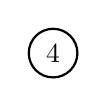
\begin{tikzpicture}[thick]
        \node[circle, draw] at (0,0 cm) {$4$};

        
    \end{tikzpicture}
    \caption[Exemplo das estruturas utilizadas na lista ordenada]{Vetores $\sorted$ e $\cert$ para
        $\now = 0$ e $\now = 3$.
        O instante $t = \frac{36}{13}$ é quando as trajetórias dos elementos $3$ e $4$ se cruzam, e
        $t = \frac{36}{11}$ é quando as trajetórias dos elementos $1$ e $4$ se cruzam.}
    \label{fig:lista:variaveis}
\end{figure}

